\section{Versuchsaufbau und Messgeräte}
Die Probe befindet sich auf einer Messapperatur in einem aufwändigen Kryostat mit fünf Glasschichten, die von außen nach Innen trennen: Luft ($T=300$K), Vakuum (thermische Isolation), Stickstoff ($T=75$K), Vakuum, Helium ($T=4,2$K), vgl. hierzu Abbildung \ref{aufbau}.

\begin{figure}[h!]
	\centering
	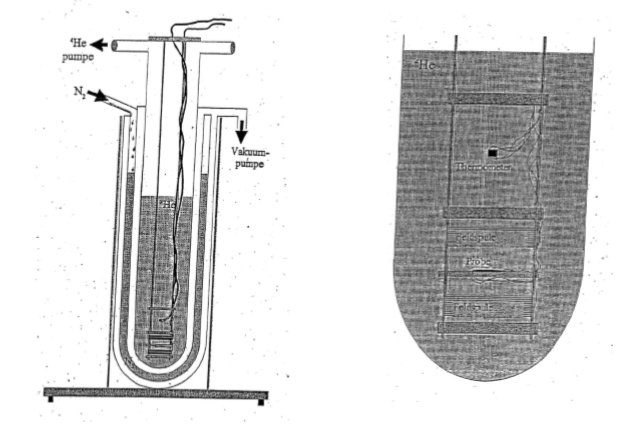
\includegraphics[height=8cm]{Aufbau.png}	
	~ %
	\caption{Messaufbau Phasenübergang Indium-Probe. \cite{Anleitung}}
	\label{aufbau}
\end{figure}

Für Indium gilt erfahrungsgemäß etwa $T_c=3,41$K, was sich unterhalb der Siedetemperatur von Helium befindet. In dem die Apperatur einem Unterdruck ausgesetzt wird, reduziert man die Temperatur (klassische Thermodynamik: Der Entzug der Verdampfungsenthalpie sorgt für eine Reduktion der Temperatur). Dadurch ist es möglich, durch bloßes Öffnen und Schließen der Ventile den Temperaturbereich von $T$=2 bis $T$=4K zu durchfahren. Währenddessen werden am Computer über einen Lock-In-Verstärker mit gespeicherter Eichkurve ständig Messwerte aufgenommen und direkt in ein R-T-Diagramm aufgetragen. Der Prozess geschieht hinreichend langsam, als dass das System im ständigen Gleichgewicht betrachtet werden kann.